% Options for packages loaded elsewhere
\PassOptionsToPackage{unicode}{hyperref}
\PassOptionsToPackage{hyphens}{url}
%
\documentclass[
]{article}
\usepackage{lmodern}
\usepackage{amsmath}
\usepackage{ifxetex,ifluatex}
\ifnum 0\ifxetex 1\fi\ifluatex 1\fi=0 % if pdftex
  \usepackage[T1]{fontenc}
  \usepackage[utf8]{inputenc}
  \usepackage{textcomp} % provide euro and other symbols
  \usepackage{amssymb}
\else % if luatex or xetex
  \usepackage{unicode-math}
  \defaultfontfeatures{Scale=MatchLowercase}
  \defaultfontfeatures[\rmfamily]{Ligatures=TeX,Scale=1}
\fi
% Use upquote if available, for straight quotes in verbatim environments
\IfFileExists{upquote.sty}{\usepackage{upquote}}{}
\IfFileExists{microtype.sty}{% use microtype if available
  \usepackage[]{microtype}
  \UseMicrotypeSet[protrusion]{basicmath} % disable protrusion for tt fonts
}{}
\makeatletter
\@ifundefined{KOMAClassName}{% if non-KOMA class
  \IfFileExists{parskip.sty}{%
    \usepackage{parskip}
  }{% else
    \setlength{\parindent}{0pt}
    \setlength{\parskip}{6pt plus 2pt minus 1pt}}
}{% if KOMA class
  \KOMAoptions{parskip=half}}
\makeatother
\usepackage{xcolor}
\IfFileExists{xurl.sty}{\usepackage{xurl}}{} % add URL line breaks if available
\IfFileExists{bookmark.sty}{\usepackage{bookmark}}{\usepackage{hyperref}}
\hypersetup{
  pdftitle={Diversity and Inclusion Overview},
  pdfauthor={Philippe J.S. De Brouwer},
  hidelinks,
  pdfcreator={LaTeX via pandoc}}
\urlstyle{same} % disable monospaced font for URLs
\usepackage[margin=1in]{geometry}
\usepackage{graphicx}
\makeatletter
\def\maxwidth{\ifdim\Gin@nat@width>\linewidth\linewidth\else\Gin@nat@width\fi}
\def\maxheight{\ifdim\Gin@nat@height>\textheight\textheight\else\Gin@nat@height\fi}
\makeatother
% Scale images if necessary, so that they will not overflow the page
% margins by default, and it is still possible to overwrite the defaults
% using explicit options in \includegraphics[width, height, ...]{}
\setkeys{Gin}{width=\maxwidth,height=\maxheight,keepaspectratio}
% Set default figure placement to htbp
\makeatletter
\def\fps@figure{htbp}
\makeatother
\setlength{\emergencystretch}{3em} % prevent overfull lines
\providecommand{\tightlist}{%
  \setlength{\itemsep}{0pt}\setlength{\parskip}{0pt}}
\setcounter{secnumdepth}{5}
\usepackage{tikz}
\usepackage{lipsum}

\newcommand{\mybox}[4]{
    \begin{figure}[h]
        \centering
    \begin{tikzpicture}
        \node[anchor=text,text width=\columnwidth-1.2cm, draw, rounded corners, line width=1pt, fill=#3, inner sep=5mm] (big) {\\#4};
        \node[draw, rounded corners, line width=.5pt, fill=#2, anchor=west, xshift=5mm] (small) at (big.north west) {#1};
    \end{tikzpicture}
    \end{figure}
}
\usepackage{float}
\usepackage{booktabs}
\usepackage{longtable}
\usepackage{array}
\usepackage{multirow}
\usepackage{wrapfig}
\usepackage{colortbl}
\usepackage{pdflscape}
\usepackage{tabu}
\usepackage{threeparttable}
\usepackage{threeparttablex}
\usepackage[normalem]{ulem}
\usepackage{makecell}
\usepackage{xcolor}
\ifluatex
  \usepackage{selnolig}  % disable illegal ligatures
\fi

\title{Diversity and Inclusion Overview}
\author{Philippe J.S. De Brouwer}
\date{18/09/2021}

\begin{document}
\maketitle
\begin{abstract}
This document offers an extract of the capabilities of the software
library \{div\} focused at creating insight in the data at highest level
(comparing teams or business divisions) -- details and other (more
actinable insight) are in other reports. This report can also be used to
get a feeling of what level of diversity is realistic to achieve without
forcing it (i.e.~by honestly promoting the best suited person).
\end{abstract}

{
\setcounter{tocdepth}{2}
\tableofcontents
}
\hypertarget{the-team}{%
\section{The Team}\label{the-team}}

This analysis is based on computer generated data and is not based on
any real team of any company. For the purpose of this report the
following built-in biases and assumptions are used:

\begin{itemize}
\tightlist
\item
  Seed for the random generator in R (statistical software): 1928
\item
  Total number of staff: 750
\item
  Gender categories used: F, M, O
\item
  Prior probabilities of those genders: 0.4, 0.58, 0.02
\item
  Respective salary bias built in for those genders: 1, 1.1, 1
\item
  Types of roles used: sales, analytics
\item
  Probabilities for those roles: 0.6, 0.4
\item
  Citizenships used: Polish, German, Italian, Indian, Other
\item
  Probabilities for those citizenships: 0.6, 0.2, 0.1, 0.05, 0.05
\item
  Grades (``career bands'\,') are numeric and we use the logic that the
  higher the number is the higher one is in the ranks of the company.
\end{itemize}

\begin{table}

\caption{\label{tab:unnamed-chunk-1}Per group: numbers and medians for salary, age}
\centering
\begin{tabular}[t]{r|l|r|r|r}
\hline
grade & gender & Nbr. & salary & age\\
\hline
 & F & 187 & 4,048 & 29\\
\cline{2-5}
 & M & 291 & 4,372 & 28\\
\cline{2-5}
\multirow{-3}{*}{\raggedleft\arraybackslash 0} & O & 6 & 4,274 & 27\\
\cline{1-5}
 & F & 97 & 8,467 & 31\\
\cline{2-5}
 & M & 108 & 9,390 & 32\\
\cline{2-5}
\multirow{-3}{*}{\raggedleft\arraybackslash 1} & O & 3 & 8,414 & 34\\
\cline{1-5}
 & F & 20 & 18,021 & 35\\
\cline{2-5}
\multirow{-2}{*}{\raggedleft\arraybackslash 2} & M & 27 & 19,666 & 33\\
\cline{1-5}
 & F & 5 & 38,219 & 40\\
\cline{2-5}
\multirow{-2}{*}{\raggedleft\arraybackslash 3} & M & 6 & 41,876 & 43\\
\hline
\end{tabular}
\end{table}

The result of those choices is shown in Table 1. For example the numbers
of ladies and men is different as well are their median salaries for the
same grade. Note that while the data is generated with different
categories of jobs, those have not been presented here.

\hypertarget{diversity}{%
\section{Diversity}\label{diversity}}

\hypertarget{gender-diversity}{%
\subsection{Gender Diversity}\label{gender-diversity}}

Diversity is measured as entropy. This is approach is:

\begin{itemize}
\tightlist
\item
  inclusive: it does not assume a binary classification, more classes
  are possible
\item
  increases belonging: it does not force us to focus on one group only
  (e.g.~percentage of women)
\item
  helps a true reflection of diversity linked to probabilities: there is
  no sharp cut-off at a certain percentage (e.g.~50\%), but a smooth
  evolution that does not penalise small --random-- changes around an
  ideal distribution.
\end{itemize}

\begin{figure}[!h]
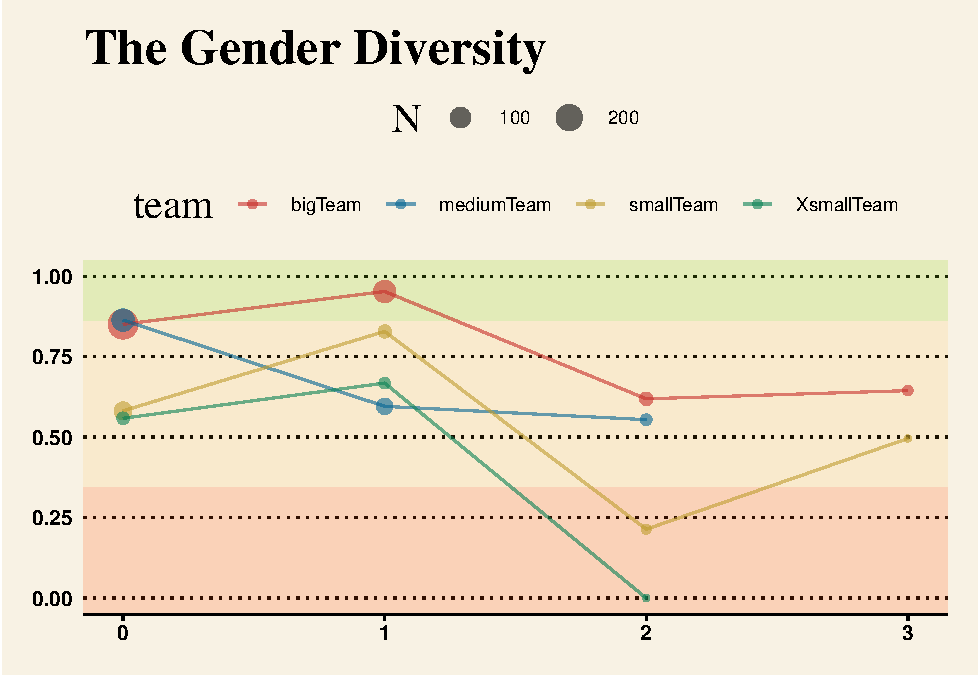
\includegraphics{div_overview_files/figure-latex/divGender-1} \caption{The diversity index per team (an index equal to one is an ideal reflection of the population. Note how for the smaller teams the index drops, while *in reality there is not more bias*. The bias built in for *all* teams is the same, only their size differs.\label{fig:divGender}}\label{fig:divGender}
\end{figure}

The results of this diversity are presented in Figure
\ref{fig:divGender}. It makes very clear that smaller teams should not
be expected to have a near-perfect split. Larger teams (even with the
same bias built in) have an easier time to be more diversified.

In general, one can observe the bias here that had been built in in the
data. While all teams had the same innate bias, it is not everywhere as
clear.

\hypertarget{other-diversity-measures}{%
\subsection{Other Diversity Measures}\label{other-diversity-measures}}

While we can measure other diversity measures than gender, it is much
harder to have a realistic benchmark. So, while we can calculate them
and present in other reports, we will not do so here.

\hypertarget{inclusion-via-pay-fairness}{%
\section{Inclusion via Pay Fairness}\label{inclusion-via-pay-fairness}}

In this sections we will investigate how much one group earns relative
to the other group. To do this we choose one category (e.g.~women,
citizens of one country, half the group of relatively younger people,
etc.) and compare the salaries of the others. This comparison is done
via a pay-ratio: we dive de median of the selected group with the median
in the remaining staff. So, if we select for example women, and the
pay-ratio is 0.9, that means that on average ladies earn 10\% less than
the other genders.

To compare those numbers, we will use the median per team over all job
categories where we can calculate such pay-ratio. While this doesn't
tell us much about outliers, it gives a fairly good impression of the
general tendency in the team.

\mybox{Pay-Ratio}{yellow!40}{brown!10}{Pay-ratios are the quotient of the median of the salaries of the control group, divided by the median salaries of all others for a given career grade and job.
\[ \text{pay-ratio} = \frac{\text{median salary control group}}{\text{median salary all others}}  \]}

\hypertarget{pay-fairness-for-gender}{%
\subsection{Pay Fairness for Gender}\label{pay-fairness-for-gender}}

Note that when the data was generated, that we did build in a bias: men
earn more than women in this data. So, we expect most pay-ratios to be
below \(1\). A pay-ratio around 0.91 is to be expected.\footnote{This is
  not exact 0.91, since we use a third gender. However, since the third
  gender has a lower probability (in our example) we should expect
  outcomes slightly above 0.91}

\begin{figure}[!h]
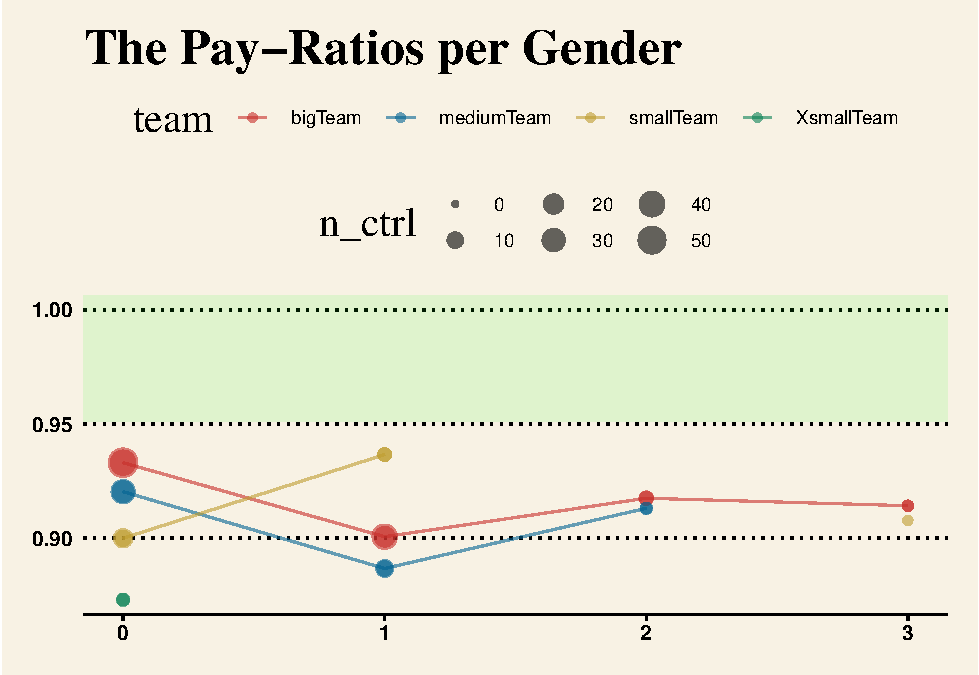
\includegraphics{div_overview_files/figure-latex/pfairnes-1} \caption{The pay-ratios per grade for each team. Note that for the smaller teams not all pay-ratios can be calculated and that for smaller teams larger deviations are possible. Finally, refer to the gender pay-bias that was built into the the data. $n\_crl$ is the number of staff in the control group (ladies in this case).}\label{fig:pfairnes}
\end{figure}

\hypertarget{pay-fairness-for-citizenship}{%
\subsection{Pay Fairness for
Citizenship}\label{pay-fairness-for-citizenship}}

Note that the generated data has no built-in bias with respect to
nationality. However, the data is generated randomly and so, we will see
certain deviations around a pay-ratio of \(1\). These variations are
random and hence not due to bias.

\begin{figure}[!h]
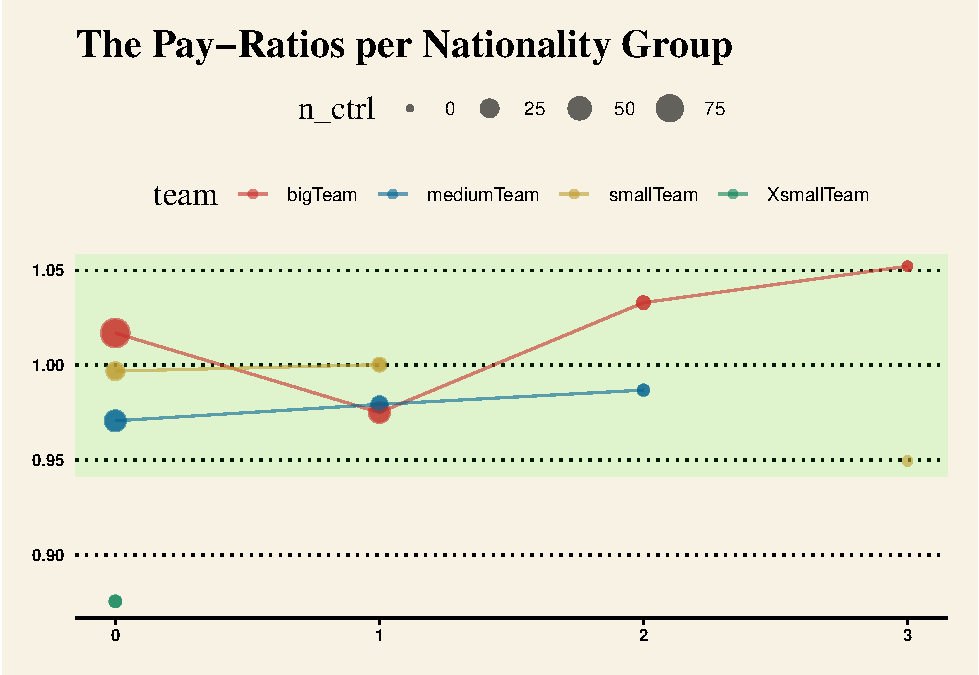
\includegraphics{div_overview_files/figure-latex/unnamed-chunk-3-1} \caption{The pay-ratios for grade per team for citizenship. Note that because there was no bias built in most numbers gravitate around 1, but deviations are possible. $n\_crl$ is the number of staff in the control group (Polish citizens)}\label{fig:unnamed-chunk-3}
\end{figure}

\hypertarget{pay-fairness-for-age}{%
\subsection{Pay Fairness for Age}\label{pay-fairness-for-age}}

Age is a continuous variable unlike gender or nationality (where we have
clear categories). In order to get categories here, look at all people
of the same grade and job and then order them according to age. Then we
split them into two groups: a group of younger people and a group of
older people. The younger people are our reference.

The generated data has no built-in bias with respect to age (older
people earn more). Therefore we can expect the pay-ratios to be around
1.

\begin{figure}[!h]
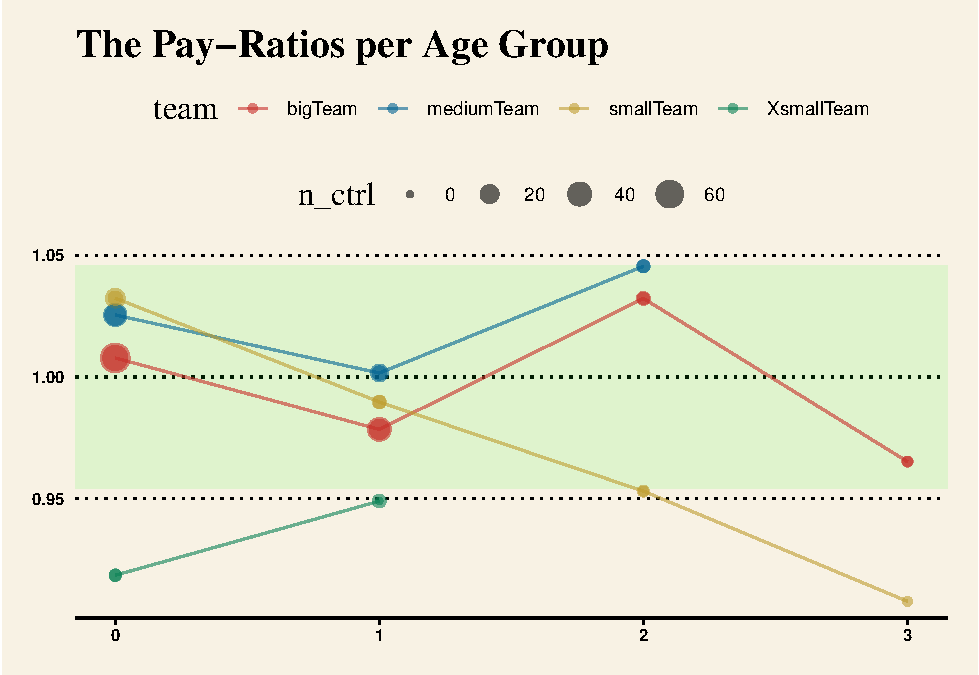
\includegraphics{div_overview_files/figure-latex/unnamed-chunk-4-1} \caption{The pay-ratios for grade per team for age. The relatively younger people are our control group. Note that a bias was built into the data. $n\_crl$ is the number of staff in the control group (younger employees)}\label{fig:unnamed-chunk-4}
\end{figure}

Note that in this particular example, the absence of innate bias is only
clearly visible in the larger groups (grade 0), where we have more
people. The higher grades, and hence smaller groups seem to show a
picture where younger people are underpaid.

This means that even if the team-leader is not biased, that randomly
salary differences might appear that are not due to bias. One might in
this particular case be most inclined to address the paygaps for the
higher grades, where younger people seem to be underpaid.

\hypertarget{other-pay-fairness-measures}{%
\subsection{Other Pay Fairness
Measures}\label{other-pay-fairness-measures}}

Other variables are possible, here is a suggestion of some variables
that should not show a bias:

\begin{itemize}
\tightlist
\item
  tenure in the company
\item
  tenure in the team
\item
  university name
\item
  experience (will largely lead to the same conclusions as age)
\item
  military service
\item
  race or ethinicity
\item
  religion
\item
  etc.
\end{itemize}

Other variables, might or might not show a bias, depending on your
approach:

\begin{itemize}
\tightlist
\item
  tenure in the grade
\item
  performance rating
\item
  diploma level
\end{itemize}

\hypertarget{other-notes-on-payment}{%
\subsection{Other notes on payment}\label{other-notes-on-payment}}

\begin{itemize}
\tightlist
\item
  Fixed or variable pay? --- both are possible, so is total pay. The
  latter is maybe the bet measure.
\item
  Overtime? --- If pay is related to number of hours worked, then the
  analysis should be done based on the pay per hour.
\end{itemize}

\end{document}
